\section{Methodology\label{sec:sota.methodo}}

This section details the methodology applied to review the state of the art of \glspl{fids}.
The original article follows the \gls{slr} methodology introduced to the engineering field by \textcite{kitchenham_Guidelinesperformingsystematic_2007}.
\Gls{slr} uses analytical methods to answer research questions about the literature on a specific topic.
The update to the original article is less structured and more focused on the evolution of the field, so the methodology is adapted accordingly.


\subsection{Research Questions\label{sec:sota.methodo.questions}}

The \gls{slr} methodology recommends defining explicit research questions to structure the review
and the selection of papers.
This survey aims at evaluating \gls{fids} and their maturity, as well
as their core components, and relevant variations.
Therefore, using related and selected works, we identify the following \glspl{rq} that cover the topic of \glspl{fids}.
The questions complete and extend \Cref{rq:intro.fids} which was introduced in \Cref{chap:intro}.

\begin{subquestions}{rq:intro.fids}
    \item What are \gls{fids}?
    \begin{questions}
        \item What challenges do \gls{fids} help to cope with? \label{rq:sota.challenges}
        \item Which techniques exist to federate \gls{ml}--based detection and mitigation mechanisms? \label{rq:sota.techniques}
    \end{questions}

    \item What are the differences between \gls{fids}?
    \begin{questions}
        \item What are the key components of \gls{fids}? How do they influence the system's performance? \label{rq:sota.components}
        \item Which metrics are used to measure and compare \gls{fids}? \label{rq:sota.metrics}
    \end{questions}

    \item What is the state of the art of \gls{fids}?
    \begin{questions}
        \item What are the topics covered by the academic literature since 2016? \label{rq:sota.literature}
        \item Where was the literature published? Which research groups and communities are active in this area? \label{rq:sota.wherewho}
        \item What are open questions according to existing works? \label{rq:sota.open}
    \end{questions}
\end{subquestions}


\subsection{Search and Selection Process\label{sec:sota.methodo.search}}

% TODO: Redo in TikZ!!
\begin{figure}
  \centering
  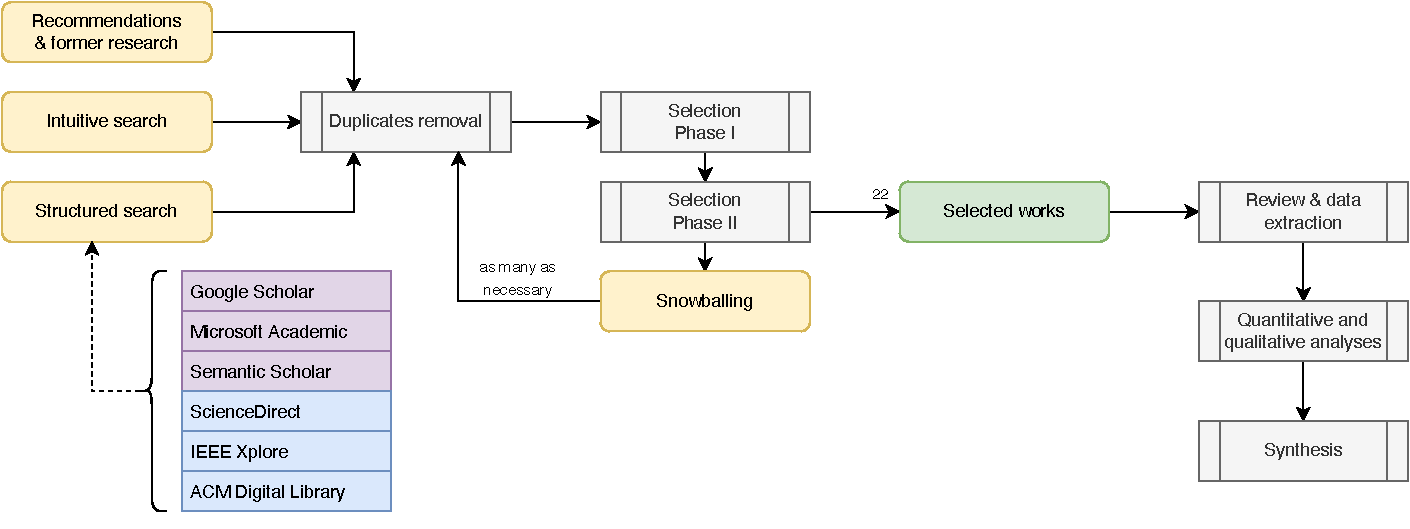
\includegraphics[width=\textwidth]{figures/methodo-survey.drawio.pdf}
  \caption{Search and selection processes}
  \label{fig:sota.methodo.original}
\end{figure}

\Cref{fig:sota.methodo.original} presents the methodology and its search, selection, and synthesis processes.
In yellow, we identify the sources of papers, in green the final selection, and in gray the processing steps of the methodology.
The tools used in the \emph{Structured search} are presented with search engines in purple, and online databases in blue.

The searching of relevant literature involves four sources: recommendations, intuitive search, structured search, and snowballing.
\begin{enumerate}[(1)]
  \item \emph{Recommendations} were given by supervisors and coworkers throughout the realization of this work.
  This initial set of relevant papers is also used as a source of snowballing for further searching.
  Moreover, we included references from an aborted survey on \emph{Collaborative security approaches}, which already yielded a substantial amount of literature by using the same methods.

  \item \emph{Intuitive search} has been performed at the beginning of the survey to get a first grasp on the topic, and to learn about the functioning of \glspl{fids}.
  At first, mostly Google Scholar has been used.

  \item \emph{Structured search} has been adopted afterward, following the principles of \gls{slr}~\cite{kitchenham_Guidelinesperformingsystematic_2007}.
  Different search engines and online databases are used for the sake of completeness, as illustrated in \Cref{fig:sota.methodo.original}. Databases can provide different results depending on their ownership.
  Search engine results differ according to the way requests are parsed, and the papers they have indexed.
  Thus, multiple sources provide more exhaustive results.
  \labelcref*{qry:method.fids} application of \gls{fl} to \glspl{ids}, and \labelcref*{qry:method.largerfids} literature addressing the topic of \gls{fids} with unusual keywords.
  \begin{queries}
    \item \texttt{("federated learning" OR "fl" OR "federated")\\ AND ("intrusion detection systems" OR "ids")} \label{qry:method.fids}
    \item \texttt{("federated" OR "collaborative")\\ AND ("detection" OR "defense" OR "mitigation")} \label{qry:method.largerfids}
  \end{queries}

  \item \emph{Snowballing} identifies relevant works that would have been missed otherwise, such as publications cited by articles of our selected corpus, or papers that refer to them.
  The related surveys identified in this work (\Cref{sec:sota.related}) contain a lot of references to technical articles, making them relevant for snowballing.
  Furthermore, as this survey proceeds with quantitative analysis of the venues and groups (\Cref{sec:sota.quanti}), it provides extended snowballing opportunities by looking at other publications in the most represented venues or research groups in the selected corpus.

\end{enumerate}

Approximately two hundred papers have been identified.
Duplicate removal is performed with Zotero which allows identifying and merging redundant items.
The selection then happens in two phases.
Firstly, the title and abstract are used to discriminate \emph{out-of-scope} papers in Phase I, along with their number of citations given the search engines, and age.
However, a paper with few citations, but interesting abstract, probably only lacks visibility.
Thus, it is moved to Phase II, which consists of a more thorough analysis of the selected works, using the \emph{three-pass} approach defined by \textcite{keshav_Howreadpaper_2007}.

After the two selection phases, 22 papers were selected, excluding the 18 initial surveys seen in \Cref{sec:sota.related}.
All present technical solution for \gls{fids}.
The challenges identified in \Cref{chap:background} were also used to either search or select papers, mostly through the \emph{intuitive search} part.


\subsection{Data Extraction and Analysis\label{sec:sota.methodo.extraction}}
% Additional section for the *new* quantitative analysis

The quantitative section of the original paper was solely based on the 22 selected papers.
However, a significant amount of literature has been published since the initial survey.
Therefore, we updated the quantitative analysis to include the latest publications on the topic.
The qualitative analysis has also been completed to a lesser extent, just enough to provide a general overview of the field's evolution.
\Cref{sec:sota.methodo.update} presents the methodology applied to update the presented results.

\begin{figure}
\centering
% TODO: Redo in TikZ!!
  \includegraphics[width=\textwidth]{example-image-golden}
  \caption{Updated selection process.}
  \label{fig:sota.methodo.update}
\end{figure}

We set up an automated collection system on Google Scholar, composed of an alert based on the search queries defined in \Cref{sec:sota.methodo.search} and automated recommendations.
The system was set up in 2021 and ran until the end of the writing of this manuscript. 
It brought 423 emails containing 2490 links after duplicate removal.
A first selection was performed on the title and abstract, yielding 238 papers.
After manual filtering, we select 158 relevant papers, which amount to 136 new publications since the original survey.

To process this new corpus, we use Litstudy~\cite{heldens_litstudyPythonpackage_2022}, a Python library providing tools to extract and analyze bibliographic data.
On the 158 selected papers, 153 only were available on Scopus, the database available in Litstudy that provides the most complete data.
The list of papers is available as appendix of this manuscript.

\paragraph{Literature distribution}

The distribution of the literature is analyzed in terms of publication year, venue, research group, and authors.
We use the properties of the document set generated by Litstudy to filter and group the papers, and use the provided Pandas adn Matplotlib bindings to analyze and plot the data.

\paragraph{Topic modeling}

Litstudy also provides tools to perform topic modeling on the text data of the papers, mainly title and abstract.
We first preprocess the text data by removing stop words, punctuation, and numbers, and then associate each word with its frequency in the corpus.
Then, we test the two main approaches of available in the literature, namely \gls{lda} and \gls{nmf}, to identify the main topics in the corpus.
The presented results have been obtained using the \gls{nmf} algorithm on 20 topics and after 2000 iterations, as it provided the most interpretable results.

